\documentclass[journal]{IEEEtran}
\usepackage{fullpage,enumitem,amsfonts,amsmath,amssymb,graphicx,cite,hyperref}

\begin{document}
\title{Personal Legal Counselor and Interpreter of the Law via Machine Learning}
\author{Derek Yan, Tianyi Wang, Patrick Chase\\
\{zhyan, tianyiw, pchase\}@stanford.edu}
\markboth{Final report for CS229, Fall 2014}
{Shell \MakeLowercase{\textit{et al.}}: Personal Legal Counselor and Interpreter of the Law via Machine Learning}
\maketitle

\begin{abstract}
The goal of this project was to predict the likelihood of winning a new legal dispute based on results of past cases. We collected over 5000 legal proceedings in the form of case briefs from the internet and used various language processing techniques to parse the raw text into feature vectors. We then used this feature vectors to train several binary classification algorithms, including Naive Bayes, random forests, logistic regression and an SVM. The SVM model achieved the highest test set accuracy of 62\%, which was an improvement over the random 50\% baseline. In this paper, we explain the details of how we transformed the raw text of the case briefs into feature vectors, and how we used them to build several models for prediction. We then discuss the results obtained by each of the models and suggest future work that could be done in the area.
\end{abstract}

\begin{keywords}
law, machine learning, case briefs, court cases.
\end{keywords}

\section{Introduction}
\IEEEPARstart{``T} he first thing we do, let's kill all the lawyers'' - William Shakespeare, 2 Henry VI, 4.2.59. 

Any major transaction, legal procedure, or patent dispute always requires an attorney-at-law in the due process. However, paying an attorney, even for a consultation, can be too expensive and out of reach for much of the population. Due to the exorbitant cost of legal action, many cases are unresolved or dropped. Our goal was to create a tool that would provide legal counsel to people who would otherwise not have access to it. In particular, our model would tell someone the probability they have of winning a given case, which would allow them to make the a better decision of whether or not to pursue further legal action. 

\begin{figure}
    \centering
    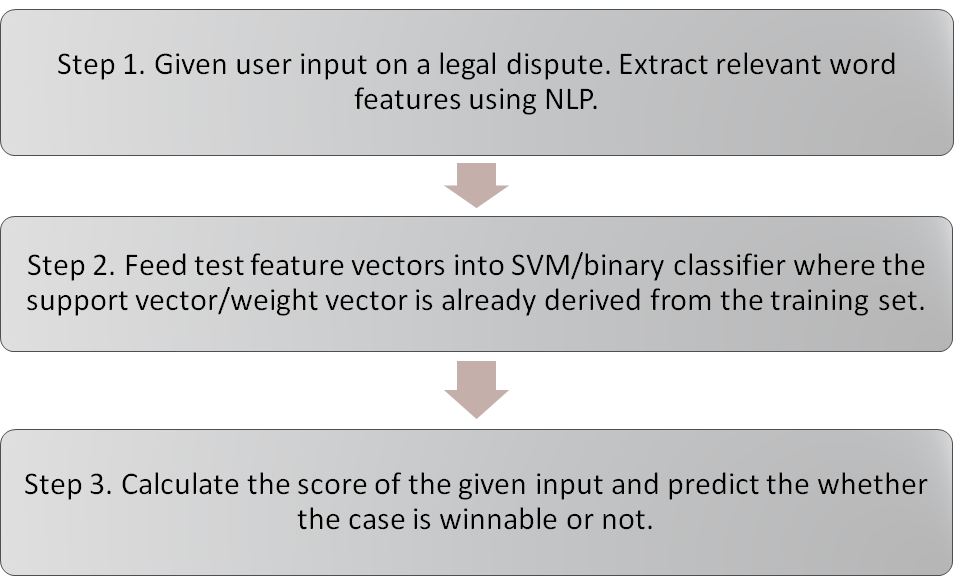
\includegraphics[width=3.5in]{flow.png}
    \caption{Processing Flow}
    \label{fig:ProcessingFlow}
\end{figure}

\section{Dataset}

\begin{figure}
    \centering
    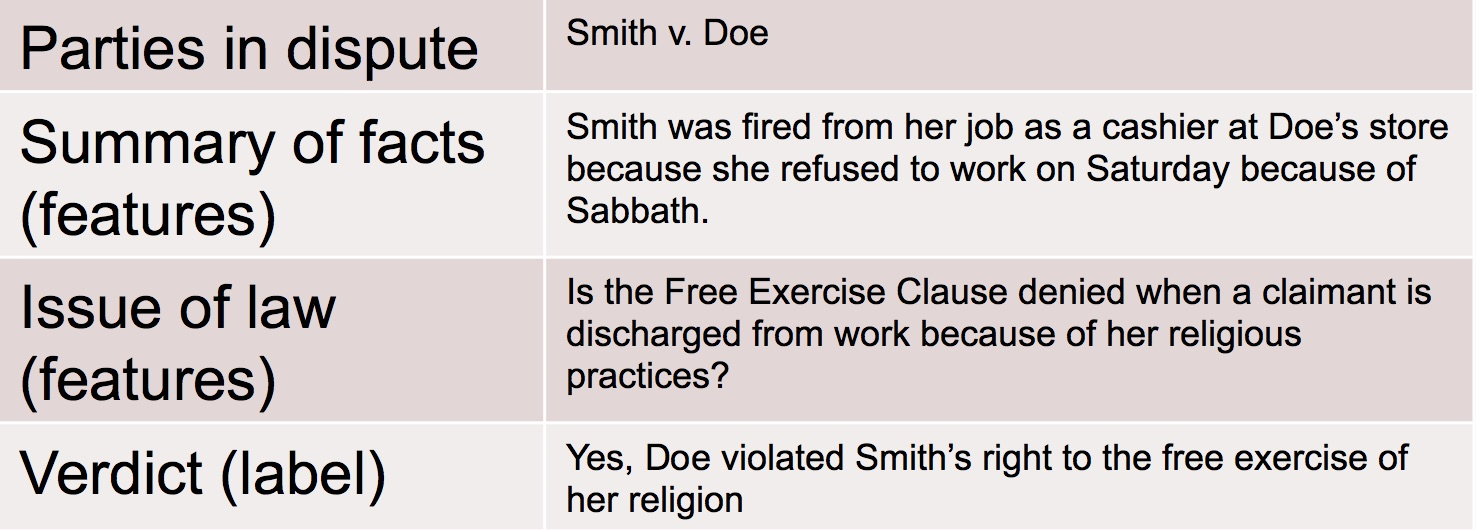
\includegraphics[width=3.5in]{exampleCaseBrief.jpg}
    \caption{Example Case Brief}
    \label{fig:ExampleCaseBrief}
\end{figure}

The processing flow is shown in the Fig. \ref{fig:ProcessingFlow}

Our dataset was obtained from \url{www.casebriefs.com}. It consisted of 5,836 legal case briefs, where each case brief was split up into four segments of text, the \textit{Parties in Dispute}, the \textit{Summary of Facts}, the \textit{Issue of Law}, and the \textit{Verdict}. Fig. \ref{fig:ExampleCaseBrief} is  an example of a very short case brief.

\section{Baseline and Oracle Results}
Before tackling the actual problem. We first considered taking the baseline and oracle results of the legal case predictor. The baseline solution was using linear regression to serve as a predictor of future cases. We used 3-grams from the input text for feature extraction.  When the new input was given, we extracted the features, and then used stochastic gradient descent to come up the learning-predictor to estimate the likelihood of the plaintiff winning the case. For the test data, we had an error rate of around 49\%. Using word features only got us around 51\% of correct prediction.

The oracle was a manual interpretation of facts and issues given a test case by the group members. We read over the facts of a legal proceeding, the interpretation of law which was under question, and used our common sense to give a probable decision. For legal matters that were not familiar to us, we would research laws of such matter and make human predictions. This would serve as our oracle. The test error would be small but still non-negligible because the group members are not of the legal profession. For our test cases of 20, we had an error rate of 10\%. 

\section{Features and Preprocessing}

First, we parsed the \textit{Verdict} section to obtain the binary labels for the cases. When the \textit{Verdict} was held, meaning the answer to the \textit{Issue of Law} was ``yes," we gave a positive label to the example, but when the answer to the \textit{Issue of Law} was ``no" we gave a negative label to the example. 

After extracting the labels, we found that there were 2099 positive cases and 3737 negative cases in our entire dataset.

\subsection{Training and Testing Data}

We then split up the data into the training and testing datasets described below.

\begin{table}[ht]
\centering
\begin{tabular}{rrr}
  \hline
& Training Dataset &	Testing Dataset\\
  \hline
Total Examples&	3800&	400 \\
Positive Examples &	1900 &	200 \\
Negative Examples &	1900 &	200 \\
   \hline
\end{tabular}
\end{table}

Since we had a sufficient amount of positive and negative examples, we chose training and testing datasets with equal number of positive and negative samples to make it easier to analyze and compare the performance of our models.

\subsection{Feature Generation}

To create the feature vectors, we used the \textit{Summary of Facts} section and \textit{Issue of Law} section. We did not use any of the text from the \textit{Verdict} section because that section was used to determine the positive or negative label.

First, we processed the raw text of the case briefs by transforming each word to its stem using the Lancaster Stemmer from the NLTK, Natural Language ToolKit \cite{Loper:2002:NNL:1118108.1118117}. We then formed a dictionary by scanning through all the words in our dataset. After forming the dictionary, we used the dictionary to represent the case briefs using the bag-of-words representation. In our representation, the $i$th element of the feature vector for an example corresponded to the number of times the $i$th stem occurred in the given case brief. In the \{key, value\} pair, key:string equals the stem (resp. n-gram) string, and value equals the count of that stem (resp. n-gram).

We also experimented with adding bigrams and trigrams to the feature vectors. For Naive Bayes, random forests, and logistic regression the huge increase in the number of features caused the algorithms to take too long or run out of memory. However, the SVM implementation, which took in a sparse matrix input, was able to run with bigrams and trigrams.

For example, if the case description was ``John was owed two weeks of pay for failing to submit his timecard''. After removing stop words and transforming words to their stems, we get \{``john'', ``owe'', ``two'', ``week'', ``pay'', ``fail'', ``submit'', ``timecard''\}. Now we count how many times each word and word gram appeared, and form the dictionary/feature vector we need: \{``john'' : 1, ``john owe'' : 1, ``john owe two'' : 1, ``owe'' : 1, ...\}

\section{Models}

For all the models we used the SciKit-Learn package \cite{scikit-learn} for python.

\subsection{Naive Bayes}

The implementation of Naive Bayes that we used assumed that the likelihood of the features was normally distributed:

\begin{equation}
\begin{aligned}
p(x_i | y) = \frac{1}{\sqrt{2 \pi \sigma_y^2}} \exp \left ( - \frac{(x_i - \mu_y)^2}{2\sigma_y^2}\right)
\end{aligned}
\end{equation}

There were no other parameters to set for Naive Bayes, so after choosing the distribution to represent the likelihood of the features, we trained our model.

\subsection{Random Forests}

When we first ran the out of the box random forest classifier from SciKit-Learn, we got an accuracy on the training set of 97\% and an accuracy on the testing set of around 53\%, illustrating that we were overfitting the training data. To remedy this issue, we set the max depth of the tree to be 6, which greatly improved our model. 

\subsection{Logistic Regression}

When modeling the outcome of a legal case with logistic regression, we had the same issue with the out of the box algorithm. We were drastically overfitting the training data, which led to a poor accuracy on the training set. To fix this issue we used a logistic regression model with L2 regularization. This decreased our training set accuracy from 99\% to 67\%, and improved the performance of the model on the testing dataset. 

\subsection{SVM}

SVM model is implemented with the LIBSVM, which support training, predicting, configuring regularization, cross validation and so on. The input feature vector used in LIBSVM is defaultly dictionary, but the keys of the \{key, value\} must be int type.
So there is a transformer that compress all the keys that appears in the output dictionaries of the feature extractor into a vector, and then use the index of each element in the compressed vector as the key of the input dictionaries of SVM. 

At first SVM was heavily favoring negatively labeled examples. i.e. it's more likely to predict new examples as negatively labeled. We fixed this by setting the gamma variable to 0.005.

Then SVM with features of word-counter gives around 99\% accuracy on the training set but around 50\% accuracy on the testing set, which indicated a overfitting problem. To solve the overfitting problem, we integrated NLTK and changed word to stem, which decreased the feature set. Another technique we used is to remove stop words, such as "to", "and" and "is", from the feature set. We also tried removing the words that have too high or too low appearance frequency from the feature set, considering those words might be meaningless, but this technique did not give quality improvement.

Our work decreased the training accuracy to around 60\% and increased the testing accuracy to around 60\%. The fact that the training error was similar to the testing error indicated that the overfitting is fixed. 

\section{Results}

The table below shows the training and testing error for each algorithm. 

\begin{table}[ht]
\centering
\begin{tabular}{rrr}
  \hline
Model & Training Set Accuracy & Testing Set Accuracy \\
  \hline
Naive Bayes &	0.9463 & 0.5879	\\
Random Forests & 0.6318 &  0.5639	 \\
L2 Reg. LogReg  &	0.6768 &	0.6080 \\
SVM & 0.6920 &  0.6210 \\
   \hline
\end{tabular}
\end{table}

Here we see that the SVM had the best performance on the testing dataset. It was able to achieve 62.1\% accuracy.

In addition, Fig.  \ref{fig:nb}, Fig.  \ref{fig:rf}, Fig.  \ref{fig:logReg}, Fig.  \ref{fig:SVM}, show the confusion matrices for each classifier. In the discussion section, we compare and contrast these results.

\begin{figure}
    \centering
    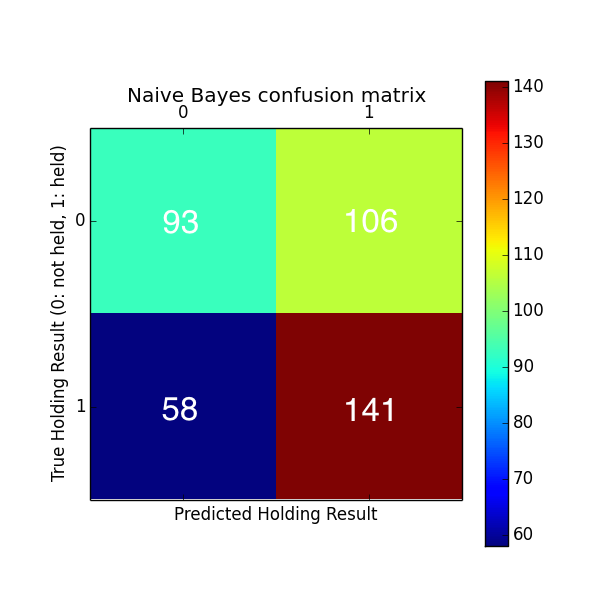
\includegraphics[width=3in]{nbConfusion.png}
    \caption{Naive Bayes Confusion Matrix}
    \label{fig:nb}
\end{figure}

\begin{figure}
    \centering
    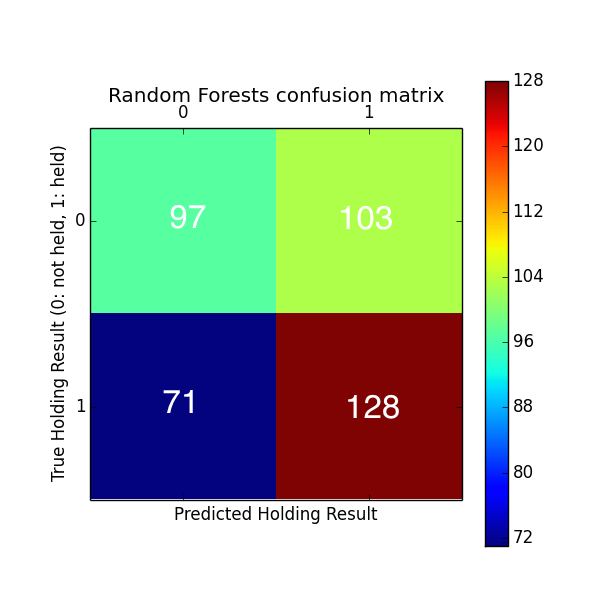
\includegraphics[width=3in]{rfConfusion.png}
    \caption{Random Forest Confusion Matrix}
    \label{fig:rf}
\end{figure}

\begin{figure}
    \centering
    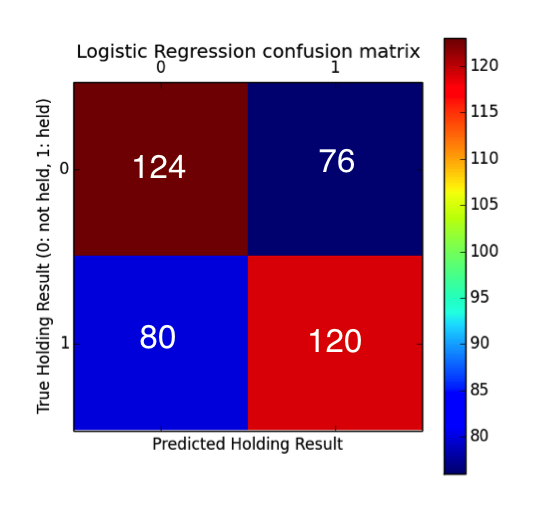
\includegraphics[width=3in]{logregConfusion.png}
    \caption{L2 Logistic Regression Confusion Matrix}
    \label{fig:logReg}
\end{figure}

\begin{figure}
    \centering
    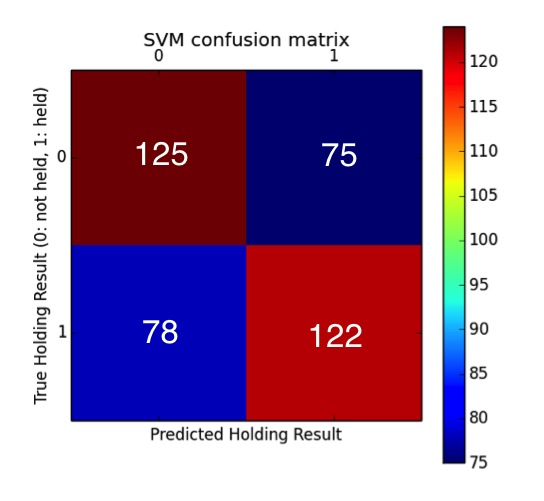
\includegraphics[width=3in]{svmConfusion.png}
    \caption{SVM Confusion Matrix}
    \label{fig:SVM}
\end{figure}

\begin{figure}
    \centering
    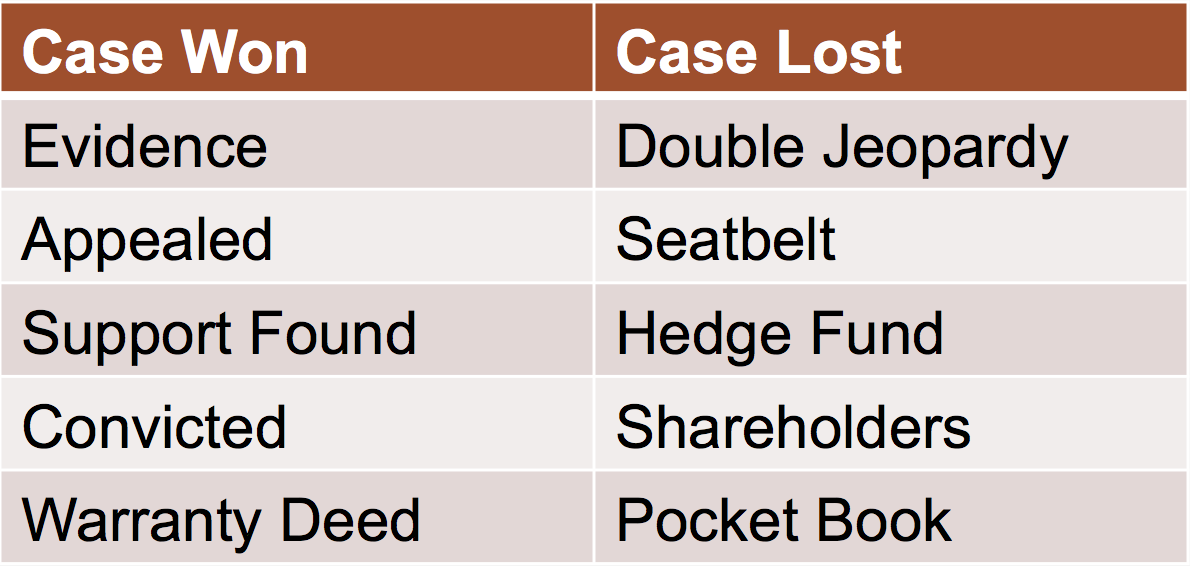
\includegraphics[width=3in]{mostIndicativeFeatures.png}
    \caption{Most Indicative Features}
    \label{fig:msf}
\end{figure}

\section{Discussion}

\subsection{Most Indicative Features}

To determine the most indicative features, we looked at the top five coefficients of the logistic regression model with the largest positive magnitude and the top five features with the largest negative magnitude. After mapping these stems back to their original words, we created the table illustrated in Fig. \ref{fig:msf}. We do see some interesting domain specific words come up, such as "evidence." It makes sense that the frequency of a word like "evidence" in the case brief would lead to a larger probability of winning the case because there is likely more evidence for the plaintiff. 

\subsection{Comparison of Models}

The confusion matrices give more information about how the binary classifier performed and make it easier to compare the four models. Both the Naive Bayes model and the random forest model have a very large number of false positives. A false positive in this case would be a bad result because you would advise someone to pursue legal action even when they have a large probability of losing the case. So, not only do Naive Bayes and random forests have a lower accuracy than the other two models, but they are worse because of the large number of false positives they have. In fact, the precision of each of these is less than 50\%.

In contrast, the logistic regression model and the SVM have much more balanced confusion matrices. They have about the same false positive and false negative rates. The precision of both of these models is over 62\%, which makes them much more desirable. Since the SVM has the best precision and the best accuracy, this is the best model out of the four. It's accuracy is 62.1\% and its precision is 62.5\%. 

\subsection{Analysis of Accuracy}

We believe that predicting the outcome of a legal case just from the raw text of the case brief 62\% of the time is a reasonable result for the first attempt at a very challenging problem. 

Legal proceeding labels are subjective in the sense that ruling are influenced by the sentiment of the jury and may not be captured fully in case briefs \cite{ObjectiveAndSubjective}. An oracle of manually studying a dispute and researching online to give a well-informed prediction only results in a correctness of 90\%.

The difficulty of this problem is that the legal information in the case brief is sophisticated, with many domain specific knowledge background. And our predicting output is not the normal true or false classification of the text like that in the spam email classification. What we are predicting is the relationship between the two entities in the case, the plaintiff and the defendant. The relationship is either the plaintiff defeating the defendant or the defendant defeating the plaintiff.

To address the first problem, feature set can be improved by collaborating with legal professionals to add nuances and hand-select features. With more domain specific knowledge, we can extract much more meaningful features besides the word counter.

We proposed using information extraction techniques to solve the second problem. The factor graph model is a good fit for extracting relationship between the plaintiff and the defendant. Important legal words and dependency paths between the two entities can be added as factors. And we also need entity linking to recognize mentions in the sentences. Since none of us have experience using these techniques, we did not implement these models in the current version given the time limit. 

\section{Conclusions}

The outcome of a legal dispute was predicted with an accuracy of around 62\% based on just the case brief using machine learning techniques. Past proceedings in the form of case briefs were used to extract features and labels. Feature extractor used techniques in NLP to remove word stems and map words of similar categories. The features that we used in the end were word grams with length 1, 2 and 3, and the labels were the verdicts of the proceeding. Naive Bayes, Random Forests, Logistic Regression and SVM were the four models used for prediction, and the SVM model achieved the best performance. 

\section{Related Work}

Machine Learning in law is relatively an untapped market. There currently is not a predictor based on past legal proceedings. With that being said, there are two existing websites that offer services in law through machine learning:

\textit{FindLaw.com}: A website that allows users to search for relevant lawyers based on legal needs and  provide legal counseling through a forum. A recommendation system is used for picking which lawyer is more relevant for the case at hand.

\textit{Judicata}: Mapping unstructured legal data into a generative model to empower lawyers to find the most relevant and convincing past proceedings. This information then can be used to support an argument in court.

\section{Future Work}

As mentioned in the discussion section, integrating more domain specific knowledge and using relation extraction model together with more sophisticated NLP techniques may result in a more accurate model. 

Besides, to help the users interact with our artificial counselor easily, an UI is needed. The UI should have at least two fields for users to input, case facts and issues. And the output is the predicted winning or losing.

Here is the link to the code for this project:

\url{https://github.com/yan7109/LawPredictor}

\bibliographystyle{abbrv}

\bibliography{cs229report.bib}



\end{document}

